\chapter{Insiemi}\label{cap:insiemi}

In questo capitolo costruiamo la \textbf{teoria degli insiemi} come un linguaggio del primo ordine
(Capitolo~\ref{cap:predicati}): prima in modo informale, per capire perché servono delle regole, poi in modo
formale attraverso gli \textbf{assiomi}. Vedremo poi che le operazioni tra insiemi sono la «traduzione» dei
connettivi logici, e che le tautologie del Capitolo~1 diventano proprietà degli insiemi.

% ──────────────────────────────────────────────────────────────
\section{Il linguaggio degli insiemi}\label{sec:linguaggio-insiemi}

Costruiamo un linguaggio del primo ordine in cui, variabili, accessori, connettivi e quantificatori a parte,
non ci sono costanti né lettere funzionali e c'è \textbf{un solo predicato binario}: «$\in$».

\dfn[linguaggio-insiemi]{Linguaggio della teoria degli insiemi}{
    Il linguaggio della teoria degli insiemi è $(I, \in)$, dove $\in$ è una lettera predicativa binaria.
    Se $a$ è in relazione $\in$ con $b$, cioè $a \in b$, diremo che $a$ è un \textbf{elemento} di $b$, o che
    $a$ \textbf{appartiene} a $b$. Scriveremo $a \notin b$ al posto di $\neg(a \in b)$.
}

\textbf{Informalmente}, gli insiemi saranno descritti da parentesi graffe che «contengono» qualcosa: se $a \in b$
scriveremo $b = \{a, \dots\}$, dove i puntini indicano la presenza eventuale di altri elementi.
Ad esempio, gli unici elementi dell'insieme $\{i, j\}$ sono $i$ e $j$.

Se $f(x)$ è una FBF, scrivere
\[ a = \{x \mid f(x)\} \quad \text{equivale a dire} \quad \forall x\,\big(x \in a \leftrightarrow f(x)\big), \]
il che è un modo per descrivere \textbf{tutti e soli} gli elementi di $a$.

\warning{Il paradosso di Russell}{
    Se restiamo informali giungiamo a paradossi. Supponiamo che $r = \{x \mid \neg(x \in x)\}$ sia un insieme,
    cioè che $\forall x\,\big(x \in r \leftrightarrow \neg(x \in x)\big)$. $r$ appartiene a se stesso?
    \begin{itemize}
        \item Se $r \in r$, allora $\neg(r \in r)$, perché questa è la proprietà che caratterizza gli elementi di $r$.
        \item Se $\neg(r \in r)$, allora $r$ soddisfa la proprietà dei propri elementi, quindi $r \in r$.
    \end{itemize}
    Assurdo! Il problema è aver ammesso una teoria \textbf{senza regole}, in cui troppe cose sono «insiemi».
    Servono quindi delle regole, gli \textbf{assiomi}, che dicano quali insiemi esistono.
}

% ──────────────────────────────────────────────────────────────
\section{Inclusione}\label{sec:inclusione}

Prima degli assiomi diamo due definizioni, che servono per enunciarli.

\dfn[inclusione]{Inclusione e inclusione propria}{
    Siano $x$ e $y$ insiemi. Definiamo
    \[ x \subseteq y \ \defsse\ \forall z\,(z \in x \rightarrow z \in y) \]
    \[ x \subset y \ \defsse\ (x \subseteq y) \wedge (x \neq y). \]
    Se $x \subseteq y$ diremo che $x$ è una \textbf{parte} (o \textbf{sottoinsieme}) di $y$;
    se $x \subset y$ diremo che $x$ è una \textbf{parte propria} di $y$.
}

% ──────────────────────────────────────────────────────────────
\section{Gli assiomi}\label{sec:assiomi}

\ass[estensionalita]{Estensionalità}{
    \[ \forall x, y\,\big(x = y \leftrightarrow \forall z\,(z \in x \leftrightarrow z \in y)\big) \]
    Ovvero: «due insiemi con gli stessi elementi sono lo stesso insieme». Ad esempio $\{a, b\} = \{b, a\}$ e $\{x, x\} = \{x\}$.
}

\ass[vuoto]{Insieme vuoto}{
    \[ \exists x\,\big(\forall y\ \neg(y \in x)\big) \]
    Ovvero: «esiste un insieme senza elementi».
}

\ass[coppia]{Coppia}{
    \[ \forall x, y\ \exists z\ \forall u\,\big(u \in z \leftrightarrow (u = x \vee u = y)\big) \]
    Ovvero: «dati due insiemi $x$ e $y$, esiste un insieme i cui elementi sono esattamente $x$ e $y$».
}

\ass[parti]{Parti}{
    \[ \forall x\ \exists y\ \forall z\,(z \in y \leftrightarrow z \subseteq x) \]
    Ovvero: «dato un insieme $x$, esiste l'insieme i cui elementi sono esattamente le parti di $x$».
}

\ass[unione]{Unione (unaria)}{
    \[ \forall f\ \exists u\ \forall z\,\big(z \in u \leftrightarrow \exists y\,(z \in y \wedge y \in f)\big) \]
    Ovvero: «dato un insieme $f$, esiste l'insieme i cui elementi sono esattamente gli elementi degli elementi di $f$».
}

\ass[separazione]{Separazione (o Comprensione)}{
    Sia $f$ un predicato unario. Allora
    \[ \forall x\ \exists y\ \forall z\,\big(z \in y \leftrightarrow (z \in x \wedge f(z))\big) \]
    Ovvero: «dato un insieme $x$, esiste l'insieme di tutti gli elementi di $x$ che soddisfano $f$».
}

Gli assiomi dicono che certi insiemi \textbf{esistono}; l'Estensionalità dice che sono anche \textbf{unici}.

\begin{concetto}
\begin{Proposizione}{Unicità degli insiemi dati dagli assiomi}{unicita-assiomi}
    \begin{prerequisiti}
        \dip{Assioma}{ass:estensionalita}
        \dip{Corollario}{cor:catene}
    \end{prerequisiti}
    Sia $\varphi(z)$ una FBF. Se $y$ e $y'$ sono insiemi tali che
    $\forall z\,(z \in y \leftrightarrow \varphi(z))$ e $\forall z\,(z \in y' \leftrightarrow \varphi(z))$, allora $y = y'$.
    In particolare, gli insiemi dati dagli assiomi dell'Insieme vuoto, della Coppia, delle Parti, dell'Unione e
    della Separazione sono \textbf{unici}.
\end{Proposizione}
\begin{dimostrazione}
    Per ogni $z$ abbiamo $z \in y \leftrightarrow \varphi(z) \leftrightarrow z \in y'$, quindi (concatenando)
    $\forall z\,(z \in y \leftrightarrow z \in y')$ e, per Estensionalità, $y = y'$.
    Per gli assiomi basta scegliere $\varphi$: per il vuoto $\varphi(z) = \neg(z = z)$ (sempre falsa, così
    «$z \in y \leftrightarrow \varphi(z)$» dice $\neg(z \in y)$), per la coppia $\varphi(z) = (z = x \vee z = y)$, e così via.
\end{dimostrazione}
\end{concetto}

\dfn[notazioni-assiomi]{Notazioni}{
    Grazie all'unicità possiamo dare un nome agli insiemi costruiti dagli assiomi:
    \begin{itemize}
        \item $\varnothing$ è l'\textbf{insieme vuoto};
        \item $\{x, y\}$ è la \textbf{coppia} di $x$ e $y$; se $x = y$ scriviamo $\{x\} = \{x, x\}$, detto \textbf{singleton} di $x$;
        \item $\mcP(x)$ è l'\textbf{insieme delle parti} di $x$;
        \item $\bigcup f$ è l'\textbf{unione} di $f$;
        \item $\{z \in x \mid f(z)\}$ è l'insieme degli elementi di $x$ che soddisfano $f$ (Separazione).
    \end{itemize}
}

\begin{concetto}
\begin{Lemma}{Caratterizzazione dell'insieme vuoto}{vuoto}
    \begin{prerequisiti}
        \dip{Assioma}{ass:estensionalita}
        \dip{Assioma}{ass:vuoto}
        \dip{Definizione}{def:notazioni-assiomi}
    \end{prerequisiti}
    Per ogni insieme $a$: \quad $a = \varnothing \leftrightarrow \forall z\,\neg(z \in a)$.
\end{Lemma}
\begin{dimostrazione}
    \begin{caso}{$(\rightarrow)$ Se $a = \varnothing$, allora $a$ non ha elementi}
        È l'assioma dell'Insieme vuoto: $\varnothing$ non ha elementi.
    \end{caso}
    \begin{caso}{$(\leftarrow)$ Se $a$ non ha elementi, allora $a = \varnothing$}
        Per ogni $z$ le formule $z \in a$ e $z \in \varnothing$ sono entrambe false, quindi
        $\forall z\,(z \in a \leftrightarrow z \in \varnothing)$ e, per Estensionalità, $a = \varnothing$.
    \end{caso}
\end{dimostrazione}
\end{concetto}

% ──────────────────────────────────────────────────────────────
\section{La collezione di tutti gli insiemi}\label{sec:russell}

Grazie agli assiomi non è più possibile costruire l'insieme di Russell.

\begin{concetto}
\begin{Teorema}{La collezione di tutti gli insiemi non è un insieme}{russell}
    \begin{prerequisiti}
        \dip{Assioma}{ass:separazione}
        \dip{Proposizione}{prop:terzoescluso}
        \dip{Proposizione}{prop:noncontraddizione}
    \end{prerequisiti}
    Non esiste un insieme $I$ tale che $\forall x\,(x \in I)$.
\end{Teorema}
\begin{dimostrazione}
    Per assurdo, sia $I$ un insieme che contiene tutti gli insiemi. Per l'assioma di \textbf{Separazione} esiste l'insieme
    \[ R = \{x \mid x \in I \wedge \neg(x \in x)\}. \]
    Poiché $R$ è un insieme, $R \in I$. Per il terzo escluso $R \in R$ oppure $R \notin R$: vediamo i due casi.
    \begin{caso}{Caso $R \in R$}
        Gli elementi di $R$ soddisfano $\neg(x \in x)$, quindi $R \notin R$.
    \end{caso}
    \begin{caso}{Caso $R \notin R$}
        Allora $R$ soddisfa $R \in I \wedge \neg(R \in R)$, cioè la proprietà che definisce $R$, quindi $R \in R$.
    \end{caso}
    In entrambi i casi si ottiene $R \in R \wedge R \notin R$, contro il principio di non contraddizione. Assurdo.
\end{dimostrazione}
\end{concetto}

% ──────────────────────────────────────────────────────────────
\section{Operazioni tra insiemi}\label{sec:operazioni}

\dfn[unione-binaria]{Unione binaria}{
    Siano $x$ e $y$ insiemi. Definiamo l'\textbf{unione} di $x$ e $y$ come
    \[ x \cup y := \bigcup\{x, y\}. \]
}

\dfn[intersezione]{Intersezione unaria e binaria}{
    Sia $f$ un insieme. Definiamo l'\textbf{intersezione} di $f$ come
    \[ \bigcap f := \{z \in \textstyle\bigcup f \mid \forall y\,(y \in f \rightarrow z \in y)\}. \]
    Siano $x$ e $y$ insiemi. Definiamo l'\textbf{intersezione} di $x$ e $y$ come $x \cap y := \bigcap\{x, y\}$.
}

\dfn[differenza]{Differenza insiemistica}{
    Siano $x$ e $y$ insiemi. Definiamo la \textbf{differenza} tra $x$ e $y$ come
    \[ x \setminus y := \{z \in x \mid \neg(z \in y)\}, \]
    cioè «l'insieme di tutti gli elementi di $x$ che non sono in $y$».
}

\dfn[diff-simmetrica]{Differenza simmetrica}{
    Siano $x$ e $y$ insiemi. Definiamo la \textbf{differenza simmetrica} tra $x$ e $y$ come
    \[ x \,\Delta\, y := \{z \in x \cup y \mid z \in x \XOR z \in y\}. \]
}

Tutte queste definizioni hanno senso perché i relativi insiemi esistono grazie agli assiomi di Coppia, Unione e
Separazione. La proposizione seguente è quella che useremo in tutte le dimostrazioni: dice quando un elemento
appartiene al risultato di un'operazione.

\begin{concetto}
\begin{Proposizione}{Appartenenza alle operazioni}{appartenenza}
    \begin{prerequisiti}
        \dip{Assioma}{ass:coppia}
        \dip{Assioma}{ass:unione}
        \dip{Assioma}{ass:separazione}
        \dip{Definizione}{def:unione-binaria}
        \dip{Definizione}{def:intersezione}
        \dip{Definizione}{def:differenza}
        \dip{Definizione}{def:diff-simmetrica}
    \end{prerequisiti}
    Per ogni insieme $x$, $y$ e per ogni $z$:
    \begin{enumerate}
        \item $z \in x \cup y \leftrightarrow z \in x \vee z \in y$;
        \item $z \in x \cap y \leftrightarrow z \in x \wedge z \in y$;
        \item $z \in x \setminus y \leftrightarrow z \in x \wedge \neg(z \in y)$;
        \item $z \in x \,\Delta\, y \leftrightarrow z \in x \XOR z \in y$.
    \end{enumerate}
\end{Proposizione}
\begin{dimostrazione}
    \begin{caso}{Punto 1: unione}
        Per l'assioma dell'Unione, $z \in \bigcup\{x, y\}$ se e solo se esiste $w$ con $z \in w$ e $w \in \{x, y\}$;
        per l'assioma della Coppia $w \in \{x,y\}$ vuol dire $w = x$ oppure $w = y$. Quindi $z \in x \cup y$ se e solo se
        $z \in x$ oppure $z \in y$.
    \end{caso}
    \begin{caso}{Punto 2: intersezione}
        Per Separazione, $z \in \bigcap\{x, y\}$ se e solo se $z \in x \cup y$ e $z$ appartiene a ogni elemento di
        $\{x, y\}$, cioè $z \in x$ e $z \in y$. La condizione $z \in x \cup y$ è allora automaticamente vera.
    \end{caso}
    \begin{caso}{Punto 3: differenza}
        È la definizione, per Separazione.
    \end{caso}
    \begin{caso}{Punto 4: differenza simmetrica}
        Per Separazione, $z \in x \,\Delta\, y$ se e solo se $z \in x \cup y$ e $z \in x \XOR z \in y$; ma se
        $z \in x \XOR z \in y$ allora $z$ sta in almeno uno dei due, quindi $z \in x \cup y$ è automaticamente vera.
    \end{caso}
\end{dimostrazione}
\end{concetto}

\textbf{Operazioni insiemistiche e connettivi logici.} La proposizione mostra che ogni operazione
\textbf{traduce} un connettivo:

\begin{table}[H]
\centering
\renewcommand{\arraystretch}{1.4}
\begin{tabular}{c|c|l}
\intestazione \textbf{Insiemi} & \textbf{Logica} & \textbf{Perché} \\ \hline
$=$ & $\leftrightarrow$ & Estensionalità: $x = y \leftrightarrow \forall z\,(z \in x \leftrightarrow z \in y)$ \\
$\subseteq$ & $\rightarrow$ & $x \subseteq y \leftrightarrow \forall z\,(z \in x \rightarrow z \in y)$ \\
$\cup$ & $\vee$ & $z \in x \cup y \leftrightarrow z \in x \vee z \in y$ \\
$\cap$ & $\wedge$ & $z \in x \cap y \leftrightarrow z \in x \wedge z \in y$ \\
$\Delta$ & XOR & $z \in x \,\Delta\, y \leftrightarrow z \in x \XOR z \in y$ \\
$\setminus$ & $\neg$ & $z \in x \setminus y \leftrightarrow z \in x \wedge \neg(z \in y)$ \\
\end{tabular}
\caption{Traduzione tra operazioni insiemistiche e connettivi.}
\end{table}

Perché per $\neg$ serve la differenza, e non il «complementare» $\{x \mid \neg(x \in a)\}$? Perché quest'ultimo non è un insieme.

\begin{concetto}
\begin{Corollario}{Il complementare assoluto non è un insieme}{complementare}
    \begin{prerequisiti}
        \dip{Teorema}{teo:russell}
        \dip{Proposizione}{prop:appartenenza}
        \dip{Proposizione}{prop:terzoescluso}
    \end{prerequisiti}
    Sia $a$ un insieme. Non esiste un insieme $c$ tale che $\forall x\,\big(x \in c \leftrightarrow \neg(x \in a)\big)$.
\end{Corollario}
\begin{dimostrazione}
    Se $c$ esistesse, allora per ogni $x$ avremmo $x \in c \cup a \leftrightarrow \neg(x \in a) \vee x \in a$, che è sempre
    vera per il terzo escluso. Quindi $c \cup a$ conterrebbe tutti gli insiemi, contro il Teorema~\ref{teo:russell}.
\end{dimostrazione}
\end{concetto}

% ──────────────────────────────────────────────────────────────
\section{Tautologie tradotte in proprietà degli insiemi}\label{sec:traduzioni}

Adesso possiamo usare le tautologie per ottenere formule valide nel linguaggio della teoria degli insiemi.
Il metodo è sempre lo stesso:
\begin{enumerate}
    \item per dimostrare che due insiemi $A$ e $B$ sono uguali, per \textbf{Estensionalità} basta dimostrare
          che $\forall z\,(z \in A \leftrightarrow z \in B)$;
    \item si scrive $z \in A$ con i connettivi usando la Proposizione~\ref{prop:appartenenza};
    \item si applica la tautologia corrispondente, e si torna indietro.
\end{enumerate}

\begin{concetto}
\begin{Proposizione}{Regola della doppia inclusione}{doppia-inclusione}
    \begin{prerequisiti}
        \dip{Assioma}{ass:estensionalita}
        \dip{Definizione}{def:inclusione}
        \dip{Proposizione}{prop:doppiaimp}
        \dip{Proposizione}{prop:forall-and}
        \dip{Proposizione}{prop:sostituzione}
        \dip{Corollario}{cor:catene}
    \end{prerequisiti}
    \[ \forall x, y\,\big(x = y \leftrightarrow (x \subseteq y \wedge y \subseteq x)\big) \]
\end{Proposizione}
\begin{dimostrazione}
    Prendo $x$ e $y$:
    \[
    \begin{aligned}
        x = y &\leftrightarrow \forall z\,(z \in x \leftrightarrow z \in y) && \text{(Estensionalità)}\\
        &\leftrightarrow \forall z\,\big((z \in x \rightarrow z \in y) \wedge (z \in y \rightarrow z \in x)\big) && \text{(doppia implicazione)}\\
        &\leftrightarrow \forall z\,(z \in x \rightarrow z \in y) \wedge \forall z\,(z \in y \rightarrow z \in x) && \text{(Proposizione~\ref{prop:forall-and})}\\
        &\leftrightarrow x \subseteq y \wedge y \subseteq x && \text{(definizione di $\subseteq$)}.
    \end{aligned}
    \]
\end{dimostrazione}
\end{concetto}

È il metodo più usato per dimostrare un'uguaglianza tra insiemi: si dimostrano le due inclusioni.

\begin{concetto}
\begin{Proposizione}{Transitività dell'inclusione}{transitivita-inclusione}
    \begin{prerequisiti}
        \dip{Definizione}{def:inclusione}
        \dip{Proposizione}{prop:tavole-connettivi}
    \end{prerequisiti}
    Siano $x$, $y$, $z$ insiemi. Se $x \subseteq y$ e $y \subseteq z$, allora $x \subseteq z$.
\end{Proposizione}
\begin{dimostrazione}
    Sia $w \in x$. Poiché $x \subseteq y$, abbiamo $w \in y$; poiché $y \subseteq z$, abbiamo $w \in z$.
    Quindi $\forall w\,(w \in x \rightarrow w \in z)$, cioè $x \subseteq z$. È la traduzione della transitività di
    $\rightarrow$: la formula $\big((p \rightarrow q) \wedge (q \rightarrow r)\big) \rightarrow (p \rightarrow r)$ è una tautologia.
\end{dimostrazione}
\end{concetto}

\begin{concetto}
\begin{Lemma}{Tautologie per l'inclusione}{taut-inclusione}
    \begin{prerequisiti}
        \dip{Proposizione}{prop:tavole-connettivi}
        \dip{Definizione}{def:xor-nand-nor}
        \dip{Proposizione}{prop:criterio-colonne}
        \dip{Corollario}{cor:catene}
    \end{prerequisiti}
    Le seguenti FBF sono tutte logicamente equivalenti tra loro:
    \[ p \rightarrow q \qquad (p \wedge q) \leftrightarrow p \qquad (p \vee q) \leftrightarrow q \qquad \neg(p \wedge \neg q) \qquad (p \XOR q) \leftrightarrow (q \wedge \neg p). \]
\end{Lemma}
\begin{dimostrazione}
    <<TAB:inclusione>>
    Tutte le colonne evidenziate coincidono con quella di $p \rightarrow q$.
\end{dimostrazione}
\end{concetto}

\begin{concetto}
\begin{Proposizione}{Caratterizzazioni dell'inclusione}{caratt-inclusione}
    \begin{prerequisiti}
        \dip{Lemma}{lem:taut-inclusione}
        \dip{Proposizione}{prop:appartenenza}
        \dip{Assioma}{ass:estensionalita}
        \dip{Lemma}{lem:vuoto}
        \dip{Definizione}{def:inclusione}
        \dip{Proposizione}{prop:sostituzione}
    \end{prerequisiti}
    Per ogni coppia di insiemi $x$, $y$ sono equivalenti:
    \[ x \subseteq y \ \leftrightarrow\ x \cap y = x \ \leftrightarrow\ x \cup y = y \ \leftrightarrow\ x \setminus y = \varnothing \ \leftrightarrow\ x \,\Delta\, y = y \setminus x. \]
\end{Proposizione}
\begin{dimostrazione}
    Poniamo $p$ = «$z \in x$» e $q$ = «$z \in y$». Ricordiamo che $x \subseteq y \leftrightarrow \forall z\,(p \rightarrow q)$.
    Confrontiamo ogni condizione con $x \subseteq y$, usando Estensionalità, la Proposizione~\ref{prop:appartenenza}
    e il Lemma~\ref{lem:taut-inclusione} (dentro $\forall z$, per la Proposizione~\ref{prop:sostituzione}).
    \begin{caso}{$x \subseteq y \leftrightarrow x \cap y = x$}
        $x \cap y = x \leftrightarrow \forall z\,\big((p \wedge q) \leftrightarrow p\big) \leftrightarrow \forall z\,(p \rightarrow q) \leftrightarrow x \subseteq y$.
    \end{caso}
    \begin{caso}{$x \subseteq y \leftrightarrow x \cup y = y$}
        $x \cup y = y \leftrightarrow \forall z\,\big((p \vee q) \leftrightarrow q\big) \leftrightarrow \forall z\,(p \rightarrow q) \leftrightarrow x \subseteq y$.
    \end{caso}
    \begin{caso}{$x \subseteq y \leftrightarrow x \setminus y = \varnothing$}
        Per il Lemma~\ref{lem:vuoto},
        $x \setminus y = \varnothing \leftrightarrow \forall z\,\neg(p \wedge \neg q) \leftrightarrow \forall z\,(p \rightarrow q) \leftrightarrow x \subseteq y$.
    \end{caso}
    \begin{caso}{$x \subseteq y \leftrightarrow x \,\Delta\, y = y \setminus x$}
        $x \,\Delta\, y = y \setminus x \leftrightarrow \forall z\,\big((p \XOR q) \leftrightarrow (q \wedge \neg p)\big) \leftrightarrow \forall z\,(p \rightarrow q) \leftrightarrow x \subseteq y$.
    \end{caso}
\end{dimostrazione}
\end{concetto}

\begin{concetto}
\begin{Proposizione}{Proprietà di unione, intersezione e differenza simmetrica}{prop-operazioni}
    \begin{prerequisiti}
        \dip{Proposizione}{prop:appartenenza}
        \dip{Assioma}{ass:estensionalita}
        \dip{Proposizione}{prop:commutativita}
        \dip{Proposizione}{prop:associativita}
        \dip{Proposizione}{prop:idempotenza}
        \dip{Proposizione}{prop:xorcommassoc}
    \end{prerequisiti}
    Per ogni insieme $x$, $y$, $z$:
    \begin{enumerate}
        \item \textbf{commutatività}: $x \cup y = y \cup x$, \ $x \cap y = y \cap x$, \ $x \,\Delta\, y = y \,\Delta\, x$;
        \item \textbf{associatività}: $(x \cup y) \cup z = x \cup (y \cup z)$, \ $(x \cap y) \cap z = x \cap (y \cap z)$, \
              $(x \,\Delta\, y) \,\Delta\, z = x \,\Delta\, (y \,\Delta\, z)$;
        \item \textbf{idempotenza}: $x \cup x = x$, \ $x \cap x = x$.
    \end{enumerate}
\end{Proposizione}
\begin{dimostrazione}
    Mostriamo come esempio la commutatività di $\cup$; tutte le altre sono identiche, cambiando la tautologia usata.
    Per ogni $w$:
    \[ w \in x \cup y \leftrightarrow w \in x \vee w \in y \leftrightarrow w \in y \vee w \in x \leftrightarrow w \in y \cup x, \]
    dove il passaggio centrale è la commutatività di $\vee$. Per Estensionalità $x \cup y = y \cup x$.
    Per $\cap$ si usano le proprietà di $\wedge$, per $\Delta$ quelle di XOR (Proposizione~\ref{prop:xorcommassoc});
    per l'idempotenza, $(p \vee p) \leftrightarrow p$ e $(p \wedge p) \leftrightarrow p$.
\end{dimostrazione}
\end{concetto}

\begin{concetto}
\begin{Proposizione}{Doppia negazione insiemistica}{doppia-neg-ins}
    \begin{prerequisiti}
        \dip{Proposizione}{prop:appartenenza}
        \dip{Assioma}{ass:estensionalita}
        \dip{Proposizione}{prop:demorgan}
        \dip{Proposizione}{prop:doppianeg}
        \dip{Proposizione}{prop:distributivita}
        \dip{Proposizione}{prop:neutri}
        \dip{Proposizione}{prop:caratt-inclusione}
    \end{prerequisiti}
    Per ogni coppia di insiemi $x$, $y$ vale $x \setminus (x \setminus y) = x \cap y$. In particolare
    \[ \forall x, y\,\big(y \subseteq x \rightarrow x \setminus (x \setminus y) = y\big). \]
\end{Proposizione}
\begin{dimostrazione}
    \begin{caso}{Per ogni $x$, $y$: $x \setminus (x \setminus y) = x \cap y$}
    \[
    \begin{aligned}
        x \setminus (x \setminus y) &= \{z \in x \mid \neg(z \in x \setminus y)\} = \{z \mid z \in x \wedge \neg(z \in x \wedge \neg(z \in y))\} && \text{(def.)}\\
        &= \{z \mid z \in x \wedge (\neg(z \in x) \vee z \in y)\} && \text{(De Morgan + doppia negazione)}\\
        &= \{z \mid (z \in x \wedge \neg(z \in x)) \vee (z \in x \wedge z \in y)\} && \text{(distributività di $\wedge$ rispetto a $\vee$)}\\
        &= \{z \mid z \in x \wedge z \in y\} = x \cap y && \text{($\falso \vee p \leftrightarrow p$)}.
    \end{aligned}
    \]
    \end{caso}
    \begin{caso}{Se $y \subseteq x$: $x \setminus (x \setminus y) = y$}
        Per il caso precedente $x \setminus (x \setminus y) = x \cap y$, e se $y \subseteq x$ allora
        $x \cap y = y \cap x = y$ (Proposizione~\ref{prop:caratt-inclusione}).
    \end{caso}
\end{dimostrazione}
\end{concetto}

\begin{concetto}
\begin{Proposizione}{Terzo escluso insiemistico}{terzo-escluso-ins}
    \begin{prerequisiti}
        \dip{Proposizione}{prop:appartenenza}
        \dip{Assioma}{ass:estensionalita}
        \dip{Proposizione}{prop:distributivita}
        \dip{Proposizione}{prop:terzoescluso}
        \dip{Proposizione}{prop:neutri}
        \dip{Proposizione}{prop:caratt-inclusione}
    \end{prerequisiti}
    Per ogni coppia di insiemi $x$, $y$ vale $y \cup (x \setminus y) = x \cup y$. In particolare
    \[ \forall x, y\,\big(y \subseteq x \rightarrow y \cup (x \setminus y) = x\big). \]
\end{Proposizione}
\begin{dimostrazione}
    \begin{caso}{Per ogni $x$, $y$: $y \cup (x \setminus y) = x \cup y$}
    \[
    \begin{aligned}
        y \cup (x \setminus y) &= \{z \mid z \in y \vee (z \in x \setminus y)\} = \{z \mid z \in y \vee (z \in x \wedge \neg(z \in y))\} && \text{(def.)}\\
        &= \{z \mid (z \in y \vee z \in x) \wedge (z \in y \vee \neg(z \in y))\} && \text{(distributività di $\vee$ rispetto a $\wedge$)}\\
        &= \{z \mid z \in y \vee z \in x\} = x \cup y && \text{($p \wedge \vero \leftrightarrow p$, terzo escluso)}.
    \end{aligned}
    \]
    \end{caso}
    \begin{caso}{Se $y \subseteq x$: $y \cup (x \setminus y) = x$}
        Per il caso precedente $y \cup (x \setminus y) = x \cup y$, e se $y \subseteq x$ allora $x \cup y = y \cup x = x$
        (Proposizione~\ref{prop:caratt-inclusione}).
    \end{caso}
\end{dimostrazione}
\end{concetto}

\begin{concetto}
\begin{Proposizione}{Non contraddizione insiemistica}{non-contr-ins}
    \begin{prerequisiti}
        \dip{Proposizione}{prop:appartenenza}
        \dip{Proposizione}{prop:associativita}
        \dip{Proposizione}{prop:commutativita}
        \dip{Proposizione}{prop:noncontraddizione}
        \dip{Proposizione}{prop:neutri}
        \dip{Lemma}{lem:vuoto}
    \end{prerequisiti}
    Per ogni coppia di insiemi $x$, $y$ vale $y \cap (x \setminus y) = \varnothing$.
\end{Proposizione}
\begin{dimostrazione}
    \[
    \begin{aligned}
        y \cap (x \setminus y) &= \{z \mid z \in y \wedge (z \in x \wedge \neg(z \in y))\} && \text{(def.)}\\
        &= \{z \mid (z \in y \wedge \neg(z \in y)) \wedge z \in x\} && \text{(associatività e commutatività di $\wedge$)}\\
        &= \varnothing && \text{($\falso \wedge p \leftrightarrow \falso$, Lemma~\ref{lem:vuoto})}.
    \end{aligned}
    \]
\end{dimostrazione}
\end{concetto}

\begin{concetto}
\begin{Proposizione}{Leggi di De Morgan insiemistiche}{demorgan-ins}
    \begin{prerequisiti}
        \dip{Proposizione}{prop:appartenenza}
        \dip{Assioma}{ass:estensionalita}
        \dip{Proposizione}{prop:demorgan}
        \dip{Proposizione}{prop:distributivita}
        \dip{Proposizione}{prop:sostituzione}
    \end{prerequisiti}
    Per ogni insieme $x$, $y$, $z$:
    \[ x \setminus (y \cap z) = (x \setminus y) \cup (x \setminus z) \qquad\qquad x \setminus (y \cup z) = (x \setminus y) \cap (x \setminus z). \]
\end{Proposizione}
\begin{dimostrazione}
    Siano $p$ = «$w \in x$», $q$ = «$w \in y$», $r$ = «$w \in z$».
    \begin{caso}{Prima legge: $x \setminus (y \cap z) = (x \setminus y) \cup (x \setminus z)$}
    \[
    \begin{aligned}
        x \setminus (y \cap z) &= \{w \mid p \wedge \neg(q \wedge r)\} = \{w \mid p \wedge (\neg q \vee \neg r)\} && \text{(De Morgan)}\\
        &= \{w \mid (p \wedge \neg q) \vee (p \wedge \neg r)\} && \text{(distributività)}\\
        &= \{w \mid w \in x \setminus y \vee w \in x \setminus z\} = (x \setminus y) \cup (x \setminus z).
    \end{aligned}
    \]
    \end{caso}
    \begin{caso}{Seconda legge: $x \setminus (y \cup z) = (x \setminus y) \cap (x \setminus z)$}
    È identica, usando l'altra legge di De Morgan: $p \wedge \neg(q \vee r) \leftrightarrow p \wedge (\neg q \wedge \neg r)
    \leftrightarrow (p \wedge \neg q) \wedge (p \wedge \neg r)$ (idempotenza, associatività e commutatività di $\wedge$).
    \end{caso}
\end{dimostrazione}
\end{concetto}

\begin{concetto}
\begin{Proposizione}{Distributività insiemistiche}{distributivita-ins}
    \begin{prerequisiti}
        \dip{Proposizione}{prop:appartenenza}
        \dip{Assioma}{ass:estensionalita}
        \dip{Proposizione}{prop:distributivita}
    \end{prerequisiti}
    $\cup$ e $\cap$ sono reciprocamente distributive: per ogni $x$, $y$, $z$
    \[ x \cup (y \cap z) = (x \cup y) \cap (x \cup z) \qquad\qquad x \cap (y \cup z) = (x \cap y) \cup (x \cap z). \]
\end{Proposizione}
\begin{dimostrazione}
    Poniamo $p$ = «$w \in x$», $q$ = «$w \in y$», $r$ = «$w \in z$» e traduciamo con la Proposizione~\ref{prop:appartenenza}.
    \begin{caso}{$x \cup (y \cap z) = (x \cup y) \cap (x \cup z)$}
        $w \in x \cup (y \cap z) \leftrightarrow p \vee (q \wedge r)$ e $w \in (x \cup y) \cap (x \cup z) \leftrightarrow (p \vee q) \wedge (p \vee r)$,
        equivalenti per la distributività di $\vee$ rispetto a $\wedge$. Si conclude per Estensionalità.
    \end{caso}
    \begin{caso}{$x \cap (y \cup z) = (x \cap y) \cup (x \cap z)$}
        $w \in x \cap (y \cup z) \leftrightarrow p \wedge (q \vee r)$ e $w \in (x \cap y) \cup (x \cap z) \leftrightarrow (p \wedge q) \vee (p \wedge r)$,
        equivalenti per la distributività di $\wedge$ rispetto a $\vee$. Si conclude per Estensionalità.
    \end{caso}
\end{dimostrazione}
\end{concetto}

\begin{concetto}
\begin{Proposizione}{Distributività di $\cap$ rispetto a $\Delta$}{distr-delta}
    \begin{prerequisiti}
        \dip{Proposizione}{prop:appartenenza}
        \dip{Assioma}{ass:estensionalita}
        \dip{Proposizione}{prop:criterio-colonne}
    \end{prerequisiti}
    Per ogni $x$, $y$, $z$: \quad $x \cap (y \,\Delta\, z) = (x \cap y) \,\Delta\, (x \cap z)$.
\end{Proposizione}
\begin{dimostrazione}
    Traducendo, basta che $p \wedge (q \XOR r)$ e $(p \wedge q) \XOR (p \wedge r)$ siano equivalenti:
    <<TAB:distrxor>>
    Le colonne evidenziate coincidono; si conclude per Estensionalità.
\end{dimostrazione}
\end{concetto}

\begin{concetto}
\begin{Proposizione}{Esplicitazioni della differenza simmetrica}{esplicitazioni-delta}
    \begin{prerequisiti}
        \dip{Proposizione}{prop:appartenenza}
        \dip{Assioma}{ass:estensionalita}
        \dip{Proposizione}{prop:xorespl}
    \end{prerequisiti}
    Per ogni $x$, $y$: \quad $x \,\Delta\, y = (x \setminus y) \cup (y \setminus x) = (x \cup y) \setminus (y \cap x)$.
\end{Proposizione}
\begin{dimostrazione}
    Traducendo, i tre insiemi corrispondono a $p \XOR q$, \ $(p \wedge \neg q) \vee (q \wedge \neg p)$ \ e
    $(p \vee q) \wedge \neg(q \wedge p)$, che sono equivalenti per le esplicitazioni di XOR
    (e la commutatività di $\wedge$). Si conclude per Estensionalità.
\end{dimostrazione}
\end{concetto}

% ──────────────────────────────────────────────────────────────
\section{Diagrammi di Venn}\label{sec:venn}

I \textbf{diagrammi di Venn} rappresentano tutte le possibili intersezioni tra un numero finito di insiemi,
disegnati come regioni di un rettangolo $U$. Ecco i diagrammi generali per 2, 3 e 4 insiemi.

\begin{concetto}
\begin{center}
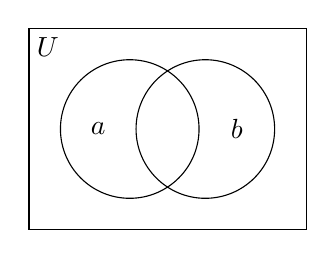
\begin{tikzpicture}[scale=0.8]
    \draw (-2.2,-1.6) rectangle (2.2,1.6); \node at (-1.9,1.3) {$U$};
    \draw (-0.6,0) circle (1.1); \draw (0.6,0) circle (1.1);
    \node at (-1.1,0) {$a$}; \node at (1.1,0) {$b$};
\end{tikzpicture}
\hspace{0.8cm}
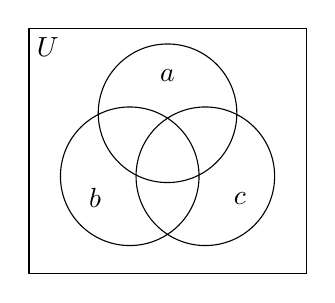
\begin{tikzpicture}[scale=0.8]
    \draw (-2.2,-2.0) rectangle (2.2,1.9); \node at (-1.9,1.6) {$U$};
    \draw (0,0.55) circle (1.1); \draw (-0.6,-0.45) circle (1.1); \draw (0.6,-0.45) circle (1.1);
    \node at (0,1.15) {$a$}; \node at (-1.15,-0.8) {$b$}; \node at (1.15,-0.8) {$c$};
\end{tikzpicture}
\hspace{0.8cm}
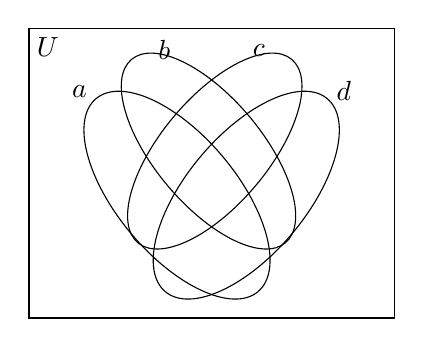
\begin{tikzpicture}[scale=0.8]
    \draw (-2.9,-2.3) rectangle (2.9,2.3); \node at (-2.6,2.0) {$U$};
    \draw (-0.55,-0.35) ellipse [x radius=2.0, y radius=0.95, rotate=-50];
    \draw (0.55,-0.35) ellipse [x radius=2.0, y radius=0.95, rotate=50];
    \draw (-0.05,0.35) ellipse [x radius=1.9, y radius=0.85, rotate=-50];
    \draw (0.05,0.35) ellipse [x radius=1.9, y radius=0.85, rotate=50];
    \node at (-2.1,1.3) {$a$}; \node at (-0.75,1.95) {$b$}; \node at (0.75,1.95) {$c$}; \node at (2.1,1.3) {$d$};
\end{tikzpicture}
\end{center}
\end{concetto}

Possono servire a visualizzare le operazioni, ad esempio l'intersezione e la differenza simmetrica:

\begin{concetto}
\begin{center}
\begin{tikzpicture}[scale=0.8]
    \draw (-2.2,-1.6) rectangle (2.2,1.6); \node at (-1.9,1.3) {$U$};
    \begin{scope} \clip (-0.6,0) circle (1.1); \fill[primary!35] (0.6,0) circle (1.1); \end{scope}
    \draw (-0.6,0) circle (1.1); \draw (0.6,0) circle (1.1);
    \node at (-1.1,0) {$a$}; \node at (1.1,0) {$b$}; \node at (0,-1.35) {$a \cap b$};
\end{tikzpicture}
\hspace{1cm}
\begin{tikzpicture}[scale=0.8]
    \draw (-2.2,-1.6) rectangle (2.2,1.6); \node at (-1.9,1.3) {$U$};
    \fill[primary!35,even odd rule] (-0.6,0) circle (1.1) (0.6,0) circle (1.1);
    \draw (-0.6,0) circle (1.1); \draw (0.6,0) circle (1.1);
    \node at (-1.1,0) {$a$}; \node at (1.1,0) {$b$}; \node at (0,-1.35) {$a \,\Delta\, b$};
\end{tikzpicture}
\end{center}
\end{concetto}

L'utilizzo più vantaggioso dei diagrammi di Venn, però, è quello di trovare \textbf{controesempi} ad alcune
relazioni insiemistiche: se i diagrammi dei due membri sono diversi, si scelgono insiemi che differiscano proprio
nelle aree in cui i diagrammi differiscono.

\begin{esempio}{$a \cup (b \,\Delta\, c) = (a \cup b) \,\Delta\, (a \cup c)$ non vale sempre}
    Disegniamo i due membri:
    \begin{center}
    \begin{tikzpicture}[scale=0.75]
        \draw (-2.2,-2.1) rectangle (2.2,1.9);
        \fill[primary!35] (0,0.55) circle (1.1);
        \fill[primary!35,even odd rule] (-0.6,-0.45) circle (1.1) (0.6,-0.45) circle (1.1);
        \draw (0,0.55) circle (1.1); \draw (-0.6,-0.45) circle (1.1); \draw (0.6,-0.45) circle (1.1);
        \node at (0,1.15) {$a$}; \node at (-1.15,-0.8) {$b$}; \node at (1.15,-0.8) {$c$};
        \node at (0,-1.85) {$a \cup (b \,\Delta\, c)$};
    \end{tikzpicture}
    \hspace{1cm}
    \begin{tikzpicture}[scale=0.75]
        \draw (-2.2,-2.1) rectangle (2.2,1.9);
        % (a ∪ b) Δ (a ∪ c) = (b Δ c) \ a
        \begin{scope}[even odd rule]
            \clip (-2.2,-2.1) rectangle (2.2,1.9) (0,0.55) circle (1.1);
            \fill[primary!35,even odd rule] (-0.6,-0.45) circle (1.1) (0.6,-0.45) circle (1.1);
        \end{scope}
        \draw (0,0.55) circle (1.1); \draw (-0.6,-0.45) circle (1.1); \draw (0.6,-0.45) circle (1.1);
        \node at (0,1.15) {$a$}; \node at (-1.15,-0.8) {$b$}; \node at (1.15,-0.8) {$c$};
        \node at (0,-1.85) {$(a \cup b) \,\Delta\, (a \cup c)$};
    \end{tikzpicture}
    \end{center}
    Sono diversi: nel secondo manca tutta la regione di $a$. Basta allora prendere $a$ con almeno un elemento
    che non sta né in $b$ né in $c$. La scelta più facile è $a = \{x\}$, $b = c = \varnothing$: allora
    \[ a \cup (b \,\Delta\, c) = a \neq \varnothing = (a \cup b) \,\Delta\, (a \cup c), \]
    e ciò dimostra che l'uguaglianza non vale sempre.
\end{esempio}

\begin{esempio}{La differenza non è associativa}
    Confrontiamo $a \setminus (b \setminus c)$ e $(a \setminus b) \setminus c$:
    \begin{center}
    \begin{tikzpicture}[scale=0.75]
        \draw (-2.2,-2.1) rectangle (2.2,1.9);
        % a \ (b \ c) = (a \ b) ∪ (a ∩ c)
        \begin{scope}
            \clip (0,0.55) circle (1.1);
            \fill[primary!35] (-2.2,-2.1) rectangle (2.2,1.9);
            \begin{scope}[even odd rule]
                \clip (-2.2,-2.1) rectangle (2.2,1.9) (0.6,-0.45) circle (1.1);
                \fill[white] (-0.6,-0.45) circle (1.1);
            \end{scope}
        \end{scope}
        \draw (0,0.55) circle (1.1); \draw (-0.6,-0.45) circle (1.1); \draw (0.6,-0.45) circle (1.1);
        \node at (0,1.15) {$a$}; \node at (-1.15,-0.8) {$b$}; \node at (1.15,-0.8) {$c$};
        \node at (0,-1.85) {$a \setminus (b \setminus c)$};
    \end{tikzpicture}
    \hspace{1cm}
    \begin{tikzpicture}[scale=0.75]
        \draw (-2.2,-2.1) rectangle (2.2,1.9);
        % (a \ b) \ c
        \begin{scope}
            \clip (0,0.55) circle (1.1);
            \fill[primary!35] (-2.2,-2.1) rectangle (2.2,1.9);
            \fill[white] (-0.6,-0.45) circle (1.1);
            \fill[white] (0.6,-0.45) circle (1.1);
        \end{scope}
        \draw (0,0.55) circle (1.1); \draw (-0.6,-0.45) circle (1.1); \draw (0.6,-0.45) circle (1.1);
        \node at (0,1.15) {$a$}; \node at (-1.15,-0.8) {$b$}; \node at (1.15,-0.8) {$c$};
        \node at (0,-1.85) {$(a \setminus b) \setminus c$};
    \end{tikzpicture}
    \end{center}
    Differiscono nella regione degli elementi che stanno in $a$ e in $c$ ma non in $b$. Prendiamo quindi
    $a = c = \{x\}$ e $b = \varnothing$: allora $a \setminus (b \setminus c) = \{x\} \setminus \varnothing = \{x\}$, mentre
    $(a \setminus b) \setminus c = \{x\} \setminus \{x\} = \varnothing$.
\end{esempio}

\begin{esempio}{L'associatività di $\Delta$ vista con i diagrammi}
    Sia $(a \,\Delta\, b) \,\Delta\, c$ sia $a \,\Delta\, (b \,\Delta\, c)$ contengono esattamente gli elementi che stanno in
    \textbf{uno solo} oppure in \textbf{tutti e tre} gli insiemi: il diagramma è lo stesso, come dimostrato nella
    Proposizione~\ref{prop:prop-operazioni}.
    \begin{center}
    \begin{tikzpicture}[scale=0.75]
        \draw (-2.2,-2.1) rectangle (2.2,1.9);
        \fill[primary!35,even odd rule] (0,0.55) circle (1.1) (-0.6,-0.45) circle (1.1) (0.6,-0.45) circle (1.1);
        \draw (0,0.55) circle (1.1); \draw (-0.6,-0.45) circle (1.1); \draw (0.6,-0.45) circle (1.1);
        \node at (0,1.15) {$a$}; \node at (-1.15,-0.8) {$b$}; \node at (1.15,-0.8) {$c$};
        \node at (0,-1.85) {$a \,\Delta\, b \,\Delta\, c$};
    \end{tikzpicture}
    \end{center}
\end{esempio}
